\begin{frame}[fragile]{Motivation}
    \vspace{-0.475cm}
    \begin{figure}
        \centering
        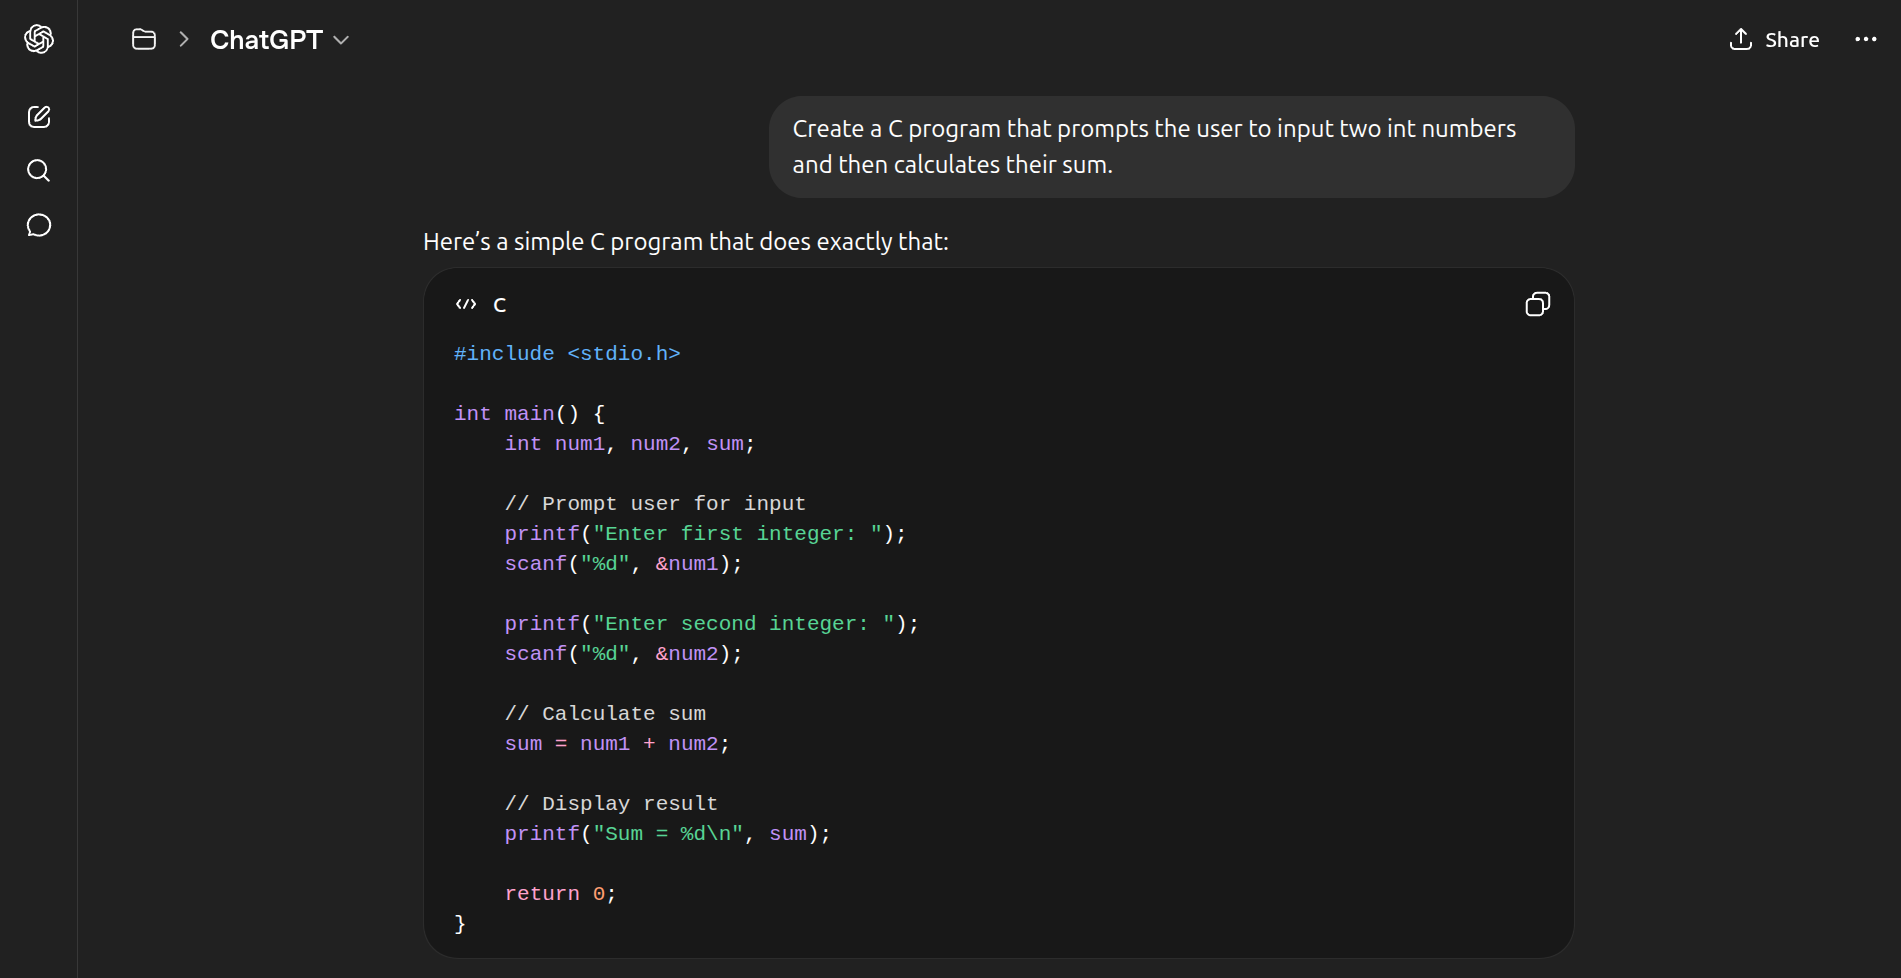
\includegraphics[width=0.97\linewidth]{images//00_motivation.png}
    \end{figure}
    \vspace{-0.37cm}
    \hspace{0.35cm}\tiny\tiny Idea from \cite{motivation_tihanyi_2024}. Generated by ChatGPT Instant 5.3 : \url{https://chatgpt.com/share/69eb9fca-a960-8388-a707-eb09f86575b7}
\end{frame}

% ===

\begin{frame}{Motivation}
    \vspace{-0.475cm}
    \begin{figure}
        \centering
        \includegraphics[width=0.75\linewidth]{images/Bildschirmfoto vom 2026-04-28 09-42-01.png}
        \includegraphics[width=0.75\linewidth]{images/Bildschirmfoto vom 2026-04-28 09-46-25.png}
    \end{figure}
    \hspace{0.35cm}\tiny\tiny MITRE: Common Weakness Enumeration (CWE) \url{https://cwe.mitre.org/top25/archive/2025/2025_cwe_top25.html}
\end{frame}

% ===

\begin{frame}{Basic \& Giaretta: Systematic Literature Review}

    \begin{columns}
    \hspace{1cm}
    
    \begin{column}{0.6\textwidth}
    \begin{exampleblock}{\textit{From Vulnerabilities to Remediation}}
    A systematic literature review of LLMs in code security covering:
    \begin{itemize}
        \item vulnerabilities introduced by LLM-generated code,
        \item LLM-based vulnerability detection and fixing,
        \item prompting strategies,
        \item data poisoning attacks.
    \end{itemize}
    \end{exampleblock}
    \end{column}

    
    \begin{column}{0.4\textwidth}
    \begin{center}
        \vspace{-0.8cm}
        \begin{tikzpicture}
            \node[
                inner sep=0pt,
                draw=black,
                line width=0.4pt,
                blur shadow={shadow blur steps=5,shadow xshift=3pt,shadow yshift=-3pt}
            ] {
                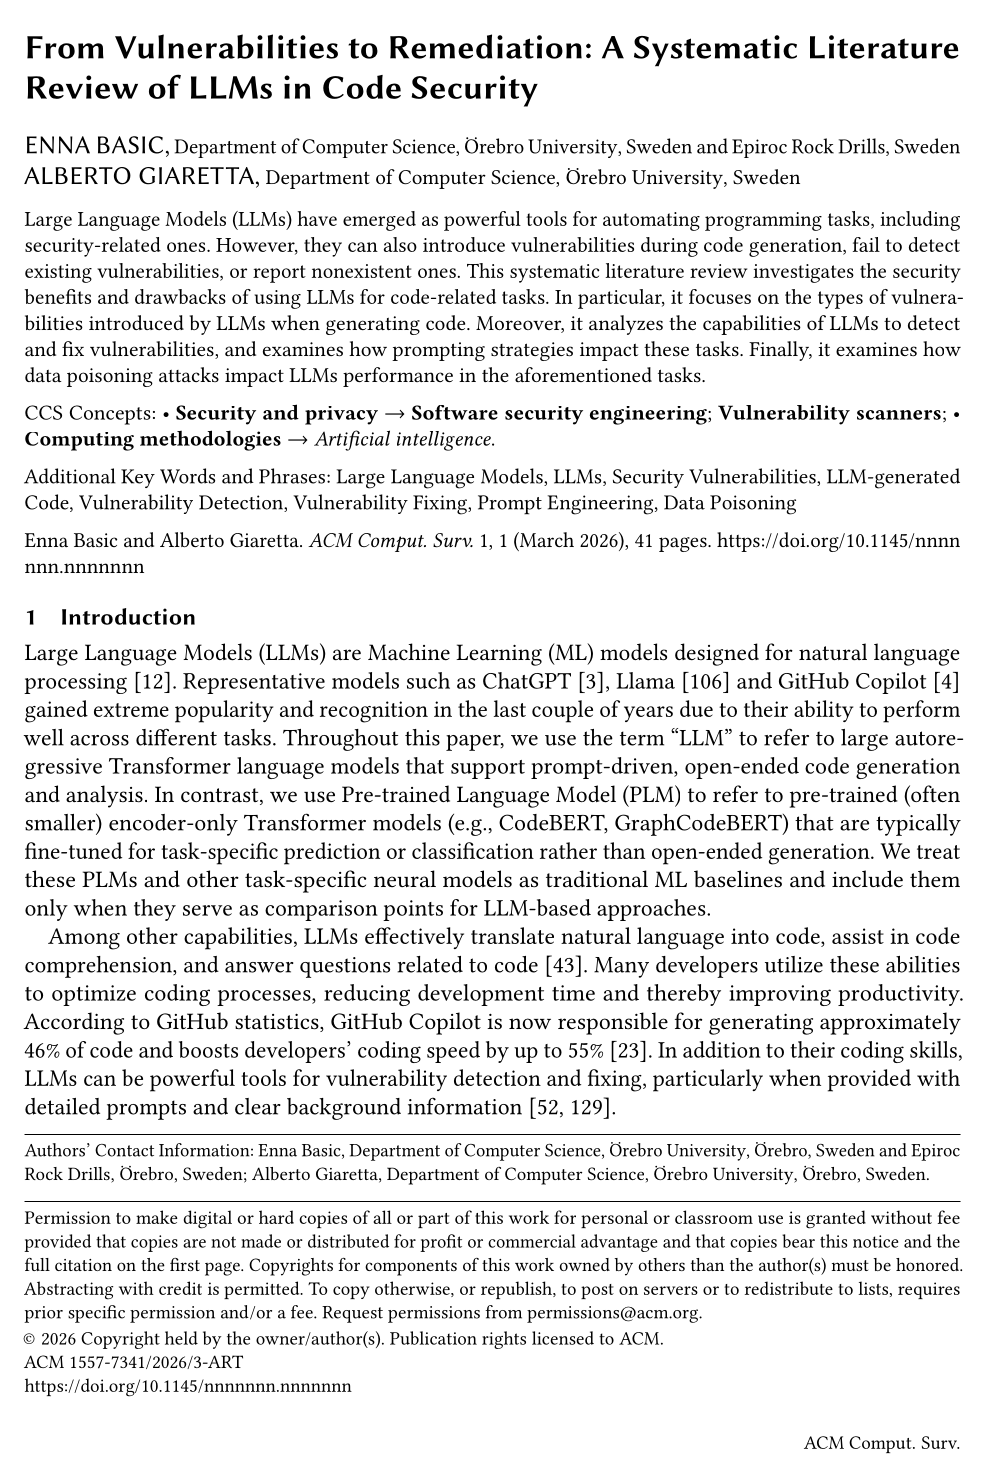
\includegraphics[width=0.75\linewidth]{images/02_SLR.png}
            };
        \end{tikzpicture}
        
        \vspace{0.025cm}
        {\scriptsize \cite{55}}
    \end{center}
    \end{column}
    
    \end{columns}

\end{frame}

% ===

\begin{frame}{Main reference: Systematic Literature Review}

    \begin{columns}
    
    \begin{column}{0.7\textwidth}
    \small
    \begin{exampleblock}{Basic \& Giaretta: \textit{From Vulnerabilities to Remediation}}
    A systematic literature review of LLMs in code security covering:
    \begin{itemize}
        \item vulnerabilities introduced by LLM-generated code,
        \item LLM-based vulnerability detection and fixing,
        \item prompting strategies,
        \item data poisoning attacks.
    \end{itemize}
    \end{exampleblock}
    \end{column}

    \hspace{-1cm}

    \begin{column}{0.3\textwidth}
    \begin{flushright}
        \vspace{-0.6cm}
        \begin{tikzpicture}
            \node[
                inner sep=0pt,
                draw=black,
                line width=0.4pt,
                blur shadow={shadow blur steps=5,shadow xshift=3pt,shadow yshift=-3pt}
            ] {
                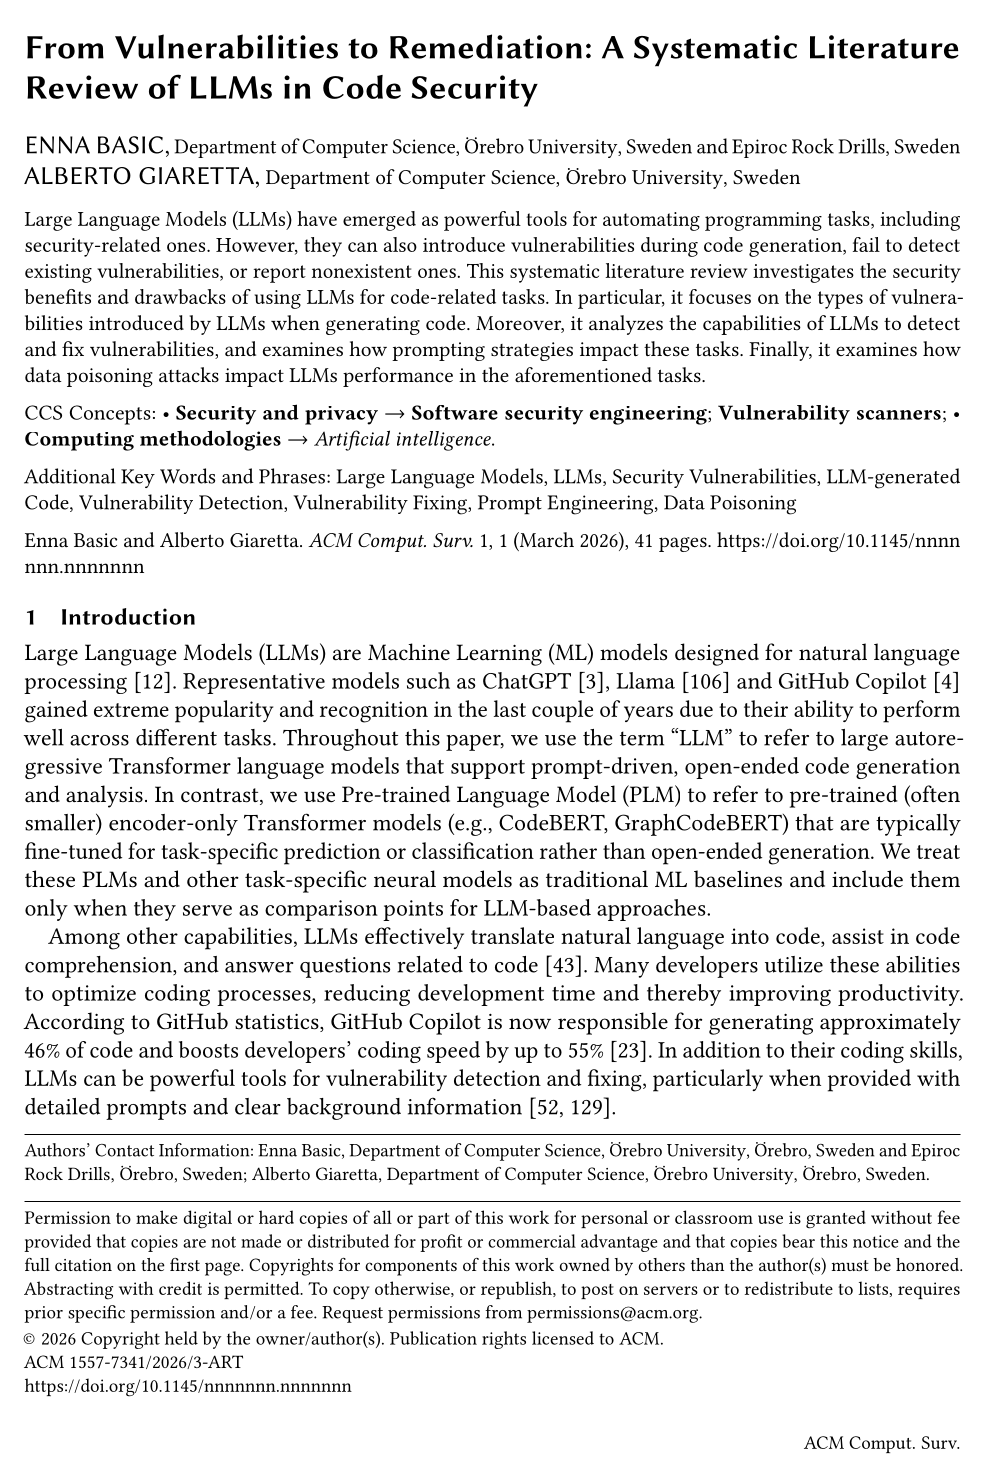
\includegraphics[width=0.9\linewidth]{images/02_SLR.png}
            };
        \end{tikzpicture}
        
        \vspace{0.025cm}
        {\tiny Systematic Literature Review \cite{55}}
    \end{flushright}
    \end{column}
    
    \end{columns}

\end{frame}

% ===

\begin{frame}
\frametitle{Main reference: Systematic Literature Review}

\begin{block}{Basic \& Giaretta: \textit{From Vulnerabilities to Remediation}}
A systematic literature review of LLMs in code security covering:
\begin{itemize}
    \item vulnerabilities introduced by LLM-generated code,
    \item LLM-based vulnerability detection and fixing,
    \item prompting strategies,
    \item data poisoning attacks.
\end{itemize}
\end{block}

\medskip

\begin{exampleblock}{Why it is useful here}
The SLR provides a structured map of the field and helps identify where a Rust-focused experiment can contribute.
\end{exampleblock}

\end{frame}

% ===

\begin{frame}
\frametitle{What the SLR covers}

\begin{columns}[T]
\begin{column}{0.46\textwidth}
\textbf{Research questions}
\begin{itemize}
    \item What vulnerabilities appear in LLM-generated code?
    \item How well do LLMs detect and fix vulnerabilities?
    \item How do prompting and poisoning affect security tasks?
\end{itemize}
\end{column}

\begin{column}{0.50\textwidth}
\textbf{Study scope}
\begin{itemize}
    \item 102 primary studies
    \item Literature through early 2026
    \item Code generation, detection, fixing, prompting, poisoning
\end{itemize}
\end{column}
\end{columns}

\bigskip

\centering
\textbf{Useful as a map, but not as a single unified experiment.}

\end{frame}

% ===


\begin{frame}
\frametitle{Vulnerability categories in LLM-generated code}

\begin{columns}[T]
\begin{column}{0.48\textwidth}
\begin{block}{Frequently reported}
\begin{itemize}
    \item Injection vulnerabilities
    \item Memory management issues
    \item File management issues
    \item Sensitive data exposure
    \item Authentication / authorization flaws
\end{itemize}
\end{block}
\end{column}

\begin{column}{0.48\textwidth}
\begin{block}{Also reported}
\begin{itemize}
    \item Weak cryptography
    \item Resource management errors
    \item Coding standard violations
    \item Error handling issues
    \item Deserialization problems
\end{itemize}
\end{block}
\end{column}
\end{columns}

\bigskip

\begin{alertblock}{Observation}
Many categories depend on language semantics. Rust changes the risk profile, especially for memory safety.
\end{alertblock}

\end{frame}

% ===

\begin{frame}
\frametitle{How previous studies evaluate LLM code security}

\begin{center}
\begin{tabular}{p{0.28\textwidth}p{0.30\textwidth}p{0.30\textwidth}}
\hline
\textbf{Experiment type} & \textbf{Strength} & \textbf{Limitation} \\
\hline
Humans vs. LLMs & Compares with human-written code & Often small or indirect \\
Controlled generation & Reproducible CWE-focused tasks & Artificial, low realism \\
Real-world code analysis & More realistic codebases & Harder to control causes \\
Mitigation / fine-tuning & Studies possible improvements & Often task- or dataset-specific \\
\hline
\end{tabular}
\end{center}

\bigskip

\centering
\textbf{The evidence depends strongly on the experimental setup.}

\end{frame}

% ===

\begin{frame}{Evaluation Approach: Humans vs. LLMs}

    \textbf{Do LLMs lead to more insecure code than human developers?}
    \begin{itemize}
        \small
        \item User studies comparing LLM-assisted developers with non assisted ones. \cite{user_study_perry_2023, user_study_sandoval_2023}
        \item Comparison quality between StackOverflow posts and LLM responses. \cite{so_firouzi_2024, so_hamer_2024}
    \end{itemize}
    
    \medskip
    
    \begin{columns}[T]
    \begin{column}{0.48\textwidth}
    \textbf{Findings}
    \begin{itemize}
        \item No consistent evidence that LLMs produce more vulnerabilities than humans.
        \item LLM-generated code can be vulnerable, but humans remain a major source of bugs.
        \item In some cases, LLM outputs are comparable or even better than common baselines (e.g., StackOverflow).
    \end{itemize}
    \end{column}
    
    \begin{column}{0.48\textwidth}
    \textbf{Limitations}
    \begin{itemize}
        \item User studies are small and task-specific.
        \item StackOverflow comparisons do not reflect real development workflows.
        \item Results depend strongly on user behavior and interaction with the model.
    \end{itemize}
    \end{column}
    \end{columns}
    
    \bigskip
    \centering
    \textbf{Key insight: LLMs do not only generate code; they change how humans write code.}

\end{frame}

% ===

\begin{frame}
\frametitle{Example: Lost at C}

\begin{block}{Sandoval et al. 2023}
A security-focused user study where students implemented a C linked-list shopping list with or without an LLM assistant.
\end{block}

\medskip

\begin{columns}[T]
\begin{column}{0.48\textwidth}
\textbf{Why it matters}
\begin{itemize}
    \item Studies actual developer interaction.
    \item Measures functionality and security.
    \item Tracks accepted LLM suggestions.
\end{itemize}
\end{column}

\begin{column}{0.48\textwidth}
\textbf{Important limitation}
\begin{itemize}
    \item Focus on C.
    \item Memory bugs are easy to express.
    \item Results may not transfer to Rust.
\end{itemize}
\end{column}
\end{columns}

\bigskip
\centering
\textbf{This motivates asking a similar question in a language with stronger safety guarantees.}

\end{frame}

% ===

\begin{frame}{Evaluation Approach: Humans vs. LLMs}

    $\Rightarrow$ \textbf{Do LLMs lead to more insecure code than human developers?}
    \vspace{0.1cm}
    \begin{itemize}
        \item User studies (2023) {\small\cite{user_study_perry_2023, user_study_sandoval_2023}} 
            % User studies comparing LLM-assisted developers with non assisted ones.
            % User study: assisted vs non-assisted developers
        \item StackOverflow comparison (2024) {\small\cite{so_firouzi_2024, so_hamer_2024}}
            % Comparison quality between StackOverflow posts and LLM responses.
            % Compare ChatGPT vs StackOverflow answers
    \end{itemize}

    % \begin{table}
    %     \centering
    %     \begin{tabular}{c|c}
    %         User studies (2023) \cite{user_study_perry_2023, user_study_sandoval_2023} 
    %         % User studies comparing LLM-assisted developers with non assisted ones.
    %         % User study: assisted vs non-assisted developers
    %         &
    %         StackOverflow comparison (2024) \cite{so_firouzi_2024, so_hamer_2024} \\
    %         % Comparison quality between StackOverflow posts and LLM responses.
    %         % Compare ChatGPT vs StackOverflow answers
    %     \end{tabular}
    % \end{table}

    \medskip

    \visible<2->{
        \textbf{Findings}
        \begin{itemize}
            \item No clear winner %(human \cite{user_study_perry_2023}, draw \cite{user_study_sandoval_2023}, LLM \cite{so_hamer_2024})
            \item Humans remain a major source of vulnerabilities
            % Sandoval: When investigating the origin of bugs within the assisted users (RQ3), 63 % of the bugs originate in code written by humans and 36 % of the bugs were present in taken suggestions.
            % Sandoval: 63% human bugs vs 36% LLM suggestions
            \item LLMs influence how developers write and review code
            % Perry: Participants with access to an AI assistant were also more likely to believe they wrote secure code, suggesting that such tools may lead users to be overconfident about security flaws in their code.
            % Perry: LLM users overconfident in security
        \end{itemize}
    }
    
    \medskip

    \visible<3->{
        \begin{alertblock}{Limitations}
            \begin{itemize}
                \item Studies may not generalize: small and very task-specific
                % User studies have N = 47-58
                % Sandoval: computer science undergraduate and graduate students
                % Firouzi: Only covered one vulnerability group -> Cryptography
                \item Results depend strongly on user behavior and interaction with the model
                % Perry: We found that those who specified task instructions, provided function declarations to use, and had the AI Assistant focus on writing helper functions generated more secure code.
            \end{itemize}
        \end{alertblock}
    }
\end{frame}

% ===

\begin{frame}{Evaluation Approach: Controlled Code Generation}

    $\Rightarrow$ \textbf{}
    \vspace{0.1cm}
    \begin{itemize}
        \item Self-defined tasks (2022-2024) {\small\cite{task_pearce_2022, task_khoury_2023, task_jamdade_2024, task_liu_2024, task_majdinasab_2024}} 
        \item Curating / Using Datasets (2022-2025) {\small\cite{dataset_siddiq_2022, dataset_asare_2023, dataset_hajipour_2024, dataset_siddiq_2024, dataset_tihanyi_2024, dataset_toth_2024, dataset_aydın_2025, dataset_gong_2025}}
    \end{itemize}

    % \begin{table}
    %     \centering
    %     \begin{tabular}{l|l}
    %         Self-defined tasks (2022-2024) \cite{task_pearce_2022, task_khoury_2023, task_jamdade_2024, task_liu_2024, task_majdinasab_2024} 
    %         % 
    %         &
    %         Curating / Using Datasets (2022-2025) \cite{dataset_siddiq_2022, dataset_asare_2023, dataset_hajipour_2024, dataset_siddiq_2024, dataset_tihanyi_2024, dataset_toth_2024, dataset_aydın_2025, dataset_gong_2025} \\
    %         % 
    %     \end{tabular}
    % \end{table}
    
    \begin{block}{Typical setup}
    Prompt an LLM to generate code for small tasks targeting specific CWEs, then analyze the output manually or with security tools.
    \end{block}
    
    \medskip
    
    \begin{columns}[T]
    \begin{column}{0.48\textwidth}
    \textbf{Findings}
    \begin{itemize}
        \item Vulnerabilities appear across many categories.
        \item Injection and input validation issues are common.
        \item Memory issues dominate in C/C++ studies.
    \end{itemize}
    \end{column}
    
    \begin{column}{0.48\textwidth}
    \textbf{Limitations}
    \begin{itemize}
        \item Small isolated tasks.
        \item Prompt wording strongly affects results.
        \item Limited representation of iterative vibe coding.
    \end{itemize}
    \end{column}
    \end{columns}
    
    \bigskip
    \centering
    \textbf{Strong control, but weaker realism.}

\end{frame}

% ===

\begin{frame}{Evaluation Approach: Controlled Code Generation}
    
    \begin{block}{Typical setup}
    Prompt an LLM to generate code for small tasks targeting specific CWEs, then analyze the output manually or with security tools.
    \end{block}
    
    \medskip
    
    \begin{columns}[T]
    \begin{column}{0.48\textwidth}
    \textbf{Findings}
    \begin{itemize}
        \item Vulnerabilities appear across many categories.
        \item Injection and input validation issues are common.
        \item Memory issues dominate in C/C++ studies.
    \end{itemize}
    \end{column}
    
    \begin{column}{0.48\textwidth}
    \textbf{Limitations}
    \begin{itemize}
        \item Small isolated tasks.
        \item Prompt wording strongly affects results.
        \item Limited representation of iterative vibe coding.
    \end{itemize}
    \end{column}
    \end{columns}
    
    \bigskip
    \centering
    \textbf{Strong control, but weaker realism.}

\end{frame}

% ===

\begin{frame}
\frametitle{Experiment type 3: Real-world code analysis}

\begin{block}{Typical setup}
Analyze LLM-generated code in repositories, projects, or larger codebases rather than isolated toy examples.
\end{block}

\medskip

\begin{columns}[T]
\begin{column}{0.48\textwidth}
\textbf{Findings}
\begin{itemize}
    \item Context matters strongly.
    \item LLMs struggle with cross-file dependencies.
    \item Security tools and LLMs often disagree.
\end{itemize}
\end{column}

\begin{column}{0.48\textwidth}
\textbf{Limitations}
\begin{itemize}
    \item Hard to attribute vulnerabilities to the LLM.
    \item Dataset construction is difficult.
    \item Evaluation is less reproducible.
\end{itemize}
\end{column}
\end{columns}

\bigskip
\centering
\textbf{More realistic, but harder to interpret.}

\end{frame}

% ===

\begin{frame}
\frametitle{Experiment type 4: Mitigation and fine-tuning}

\begin{block}{Typical setup}
Improve LLM security behavior using better prompts, iterative repair, external tools, fine-tuning, or validation loops.
\end{block}

\medskip

\begin{columns}[T]
\begin{column}{0.48\textwidth}
\textbf{Findings}
\begin{itemize}
    \item Context-rich prompts can improve results.
    \item Iterative feedback can fix some issues.
    \item Fine-tuning helps on known task distributions.
\end{itemize}
\end{column}

\begin{column}{0.48\textwidth}
\textbf{Limitations}
\begin{itemize}
    \item Improvements are often benchmark-specific.
    \item Complex vulnerabilities remain difficult.
    \item Human review is still needed.
\end{itemize}
\end{column}
\end{columns}

\bigskip
\centering
\textbf{Mitigation helps, but does not remove the need for security evaluation.}

\end{frame}

% ===

\begin{frame}

\frametitle{Research Gaps \& Limitations}

\textcolor{red}{Show new paper that I found about vibe coding}

\begin{block}{Concern}
Many experiments use small CWE-targeted tasks. This is useful, but it does not fully represent modern ``vibe coding''.
\end{block}

\medskip

\begin{columns}[T]
\begin{column}{0.48\textwidth}
\textbf{Controlled tasks}
\begin{itemize}
    \item Clear prompts
    \item Single function or file
    \item Easier evaluation
\end{itemize}
\end{column}

\begin{column}{0.48\textwidth}
\textbf{Vibe coding}
\begin{itemize}
    \item Iterative interaction
    \item Larger context
    \item User accepts, edits, and reprompts
\end{itemize}
\end{column}
\end{columns}

\bigskip
\centering
\textbf{For this seminar thesis, controlled Rust tasks are a feasible first step.}

\end{frame}

% ===

\begin{frame}
\frametitle{Gap 2: Programming languages are unevenly studied}

\textcolor{red}{Merge this with prev. slide}

\begin{exampleblock}{Why Rust is interesting}
Rust prevents many memory-safety bugs by design, but LLMs may still:
\begin{itemize}
    \item fail to produce compiling code,
    \item fight the borrow checker,
    \item use unsafe features,
    \item introduce vulnerabilities not prevented by Rust.
\end{itemize}
\end{exampleblock}

\end{frame}

% ===

\begin{frame}{Experiment Proposal}

    \begin{alertblock}{Goal}
        Determine in which contexts LLMs generate vulnerable Rust code.
    \end{alertblock}

    \medskip

    \textbf{Approach}
    \begin{itemize}
        \item Adapt controlled code-generation setup from prior work
        \item Define multiple Rust-specific tasks for 4 CWEs
        \item Evaluate outputs from two LLMs
    \end{itemize}

    \medskip

    \textbf{Key idea}
    \begin{itemize}
        \item Test whether known vulnerability patterns transfer to Rust
    \end{itemize}

\end{frame}

% ===

\begin{frame}
\frametitle{Scenario design}

\begin{block}{Each scenario should specify}
\begin{itemize}
    \item a realistic programming task,
    \item expected security property,
    \item relevant CWE,
    \item whether Rust should prevent the issue by design,
    \item evaluation criteria.
\end{itemize}
\end{block}

\medskip

\begin{exampleblock}{Example structure}
\textbf{Task:} Implement a function that receives a filename and returns file contents.\newline
\textbf{Security risk:} path traversal if user input is not restricted.\newline
\textbf{CWE:} CWE-22.\newline
\textbf{Rust protection:} not prevented by the language.
\end{exampleblock}

\end{frame}

% ===

\subsection{Experiment proposal}

\begin{frame}
\frametitle{Thesis experiment: high-level idea}

\begin{alertblock}{Goal}
Determine in which contexts LLMs generate vulnerable Rust code.
\end{alertblock}

\medskip

\begin{block}{Approach}
\begin{itemize}
    \item Select one well-cited controlled code-generation paper as methodological anchor.
    \item Choose at least four CWEs.
    \item Design multiple Rust-specific scenarios for each CWE.
    \item Evaluate outputs from two accessible LLMs.
\end{itemize}
\end{block}

\medskip

\begin{exampleblock}{Main contribution}
A small, controlled experiment that tests whether prior CWE-based findings transfer to Rust.
\end{exampleblock}

\end{frame}

% ===

\begin{frame}
\frametitle{Candidate CWEs}

\begin{center}
\begin{tabular}{p{0.18\textwidth}p{0.34\textwidth}p{0.34\textwidth}}
\hline
\textbf{CWE} & \textbf{Rust relevance} & \textbf{Possible scenario} \\
\hline
CWE-416 & Usually prevented & Store references beyond lifetime / unsafe pointer use \\
CWE-787 & Usually prevented & Write outside buffer bounds / unsafe slice indexing \\
CWE-190 & Not fully prevented & Arithmetic in release builds, size calculations \\
CWE-78 & Not prevented & Build shell command from user input \\
CWE-22 & Not prevented & Open user-controlled file path \\
CWE-20 & Not prevented & Missing validation of user-provided data \\
\hline
\end{tabular}
\end{center}

\bigskip
\centering
\textbf{Final selection: at least four CWEs, with multiple tasks per CWE.}

\end{frame}

% ===

\begin{frame}{Experiment Proposal: Core Idea}

    \textbf{Approach}
    \begin{itemize}
        \item Adapt controlled code-generation setup from \cite{task_liu_2024}
        \item Define multiple Rust-specific tasks for selected CWEs
        \item Evaluate outputs from two LLMs
    \end{itemize}
        
    \begin{columns}
    \begin{column}{0.48\textwidth}
    \begin{block}{Usually prevented by Rust}
    \begin{itemize}
        \item use-after-free
        \item null pointer dereference
        \item out-of-bounds access
        \item buffer overflow
    \end{itemize}
    \end{block}
    \end{column}
    
    \begin{column}{0.48\textwidth}
    \begin{alertblock}{Not prevented by Rust}
    \begin{itemize}
        \item integer overflow
        \item OS command injection
        \item path traversal
        \item missing input validation
    \end{itemize}
    \end{alertblock}
    \end{column}
    \end{columns}

    % \textbf{Evaluation:}
    % \begin{itemize}
    %     \item Does the code even compile?
    %     \item Are unsafe patterns used?
    % \end{itemize}

    % \begin{exampleblock}{Research Questions}
    %     \begin{enumerate}
    %         \item[RQ1] In which contexts do LLMs generate vulnerabilities in Rust?
    %         \item[RQ2] Do Rust's safety guarantees prevent typical vulnerability patterns?
    %         \item[RQ3]
    %     \end{enumerate}
    % \end{exampleblock}
\end{frame}

% ===

\begin{frame}
\frametitle{Evaluation criteria}

\begin{columns}[T]
\begin{column}{0.48\textwidth}
\textbf{Functional checks}
\begin{itemize}
    \item Does the code compile?
    \item Does it pass basic tests?
    \item Does it solve the requested task?
\end{itemize}
\end{column}

\begin{column}{0.48\textwidth}
\textbf{Security checks}
\begin{itemize}
    \item Is the target CWE present?
    \item Does the model use \fct{unsafe}?
    \item Does it rely on risky APIs or unchecked assumptions?
\end{itemize}
\end{column}
\end{columns}

\bigskip

\begin{alertblock}{Special Rust check}
For CWEs normally prevented by Rust, non-compilation is not necessarily a failure of Rust; it may be evidence that Rust blocks the vulnerable pattern.
\end{alertblock}

\end{frame}

% ===

\begin{frame}
\frametitle{Research questions}

\begin{block}{RQ1}
In which contexts do LLMs generate vulnerabilities in Rust?
\end{block}

\begin{block}{RQ2}
Do Rust's safety guarantees prevent typical LLM-generated vulnerability patterns?
\end{block}

\begin{block}{RQ3}
Do LLMs bypass Rust's safety mechanisms, for example by using \fct{unsafe} or other risky patterns?
\end{block}

\bigskip
\centering
\textbf{The experiment connects prior CWE-based evaluations with Rust-specific language guarantees.}

\end{frame}

% ===

\begin{frame}{Summary}
    
    \begin{itemize}
        \item Prior work shows that LLM-generated code can contain security vulnerabilities.
        \item Evidence depends strongly on task design, prompts, datasets, models, and languages.
        \item Rust is underrepresented, although it changes the vulnerability landscape.
        \item The thesis experiment will test selected CWEs with Rust-specific scenarios and two LLMs.
    \end{itemize}
    
    \bigskip
    
    \begin{alertblock}{Takeaway}
    The goal is not to prove that LLMs are generally safe or unsafe, but to identify \textit{where} Rust helps and \textit{where} risks remain.
    \end{alertblock}

\end{frame}

% ===

\begin{frame}
\frametitle{Backup: Why Rust changes the problem}

\begin{block}{Rust safety by default}
Rust's ownership model and borrow checker prevent many classes of memory errors without a garbage collector.
\end{block}

\begin{alertblock}{But not all vulnerabilities disappear}
Rust does not automatically prevent injection vulnerabilities, path traversal, authorization mistakes, weak cryptography, or logic errors.
\end{alertblock}

\begin{exampleblock}{Therefore}
Rust is ideal for separating vulnerabilities that are language-prevented from vulnerabilities that remain application-level problems.
\end{exampleblock}

\end{frame}

% -----------------------------------------------------------------------------
\begin{frame}
\frametitle{Backup: Unsafe Rust}

\begin{block}{Why \textbf{unsafe} matters}
\textbf{unsafe} allows operations that the compiler cannot fully verify, such as raw pointer dereferencing and calling unsafe functions.
\end{block}

\begin{alertblock}{Experiment relevance}
If an LLM uses \textbf{}{unsafe} to satisfy a task, it may bypass the safety guarantees that make Rust interesting in the first place.
\end{alertblock}

\end{frame}

% -----------------------------------------------------------------------------
\begin{frame}
\frametitle{Backup: Possible task template}

\begin{center}
\begin{tabular}{p{0.25\textwidth}p{0.60\textwidth}}
\hline
\textbf{Field} & \textbf{Example} \\
\hline
CWE & CWE-78: OS Command Injection \\
Prompt & Write a Rust function that pings a host provided by the user. \\
Expected safe behavior & Use argument-based process execution, validate host input, avoid shell string concatenation. \\
Failure pattern & \fct{Command::new("sh").arg("-c").arg(format!(...))} \\
Evaluation & Compile, tests, manual CWE inspection, unsafe/risky API usage \\
\hline
\end{tabular}
\end{center}

\end{frame}

% -----------------------------------------------------------------------------
\begin{frame}
\frametitle{Backup: Candidate models}

\begin{block}{Requirement}
Use two LLMs that are practically accessible during the thesis.
\end{block}

\begin{itemize}
    \item ChatGPT
    \item Claude
    \item Gemini
\end{itemize}

\bigskip

\begin{alertblock}{Important for validity}
The exact model version, date, prompt, and settings should be documented because model behavior changes over time.
\end{alertblock}

\end{frame}

